\section{Confiança, comprimento e custo}
\label{sec:diagnosticos}
\subsection{O escore muda. A classe fica.}
Ajustamos uma temperatura \(\tau>0\) na amostra de calibração, minimizando
a CE. Com margem \(\Delta=z_+-z_-\), o escore passa de
\(\sigma(\Delta)\) a \(\sigma(\Delta/\tau)\). A transformação mantém o
sinal de \(\Delta\), de modo que a classe e as métricas de classificação
permanecem iguais no limiar de 50\%.

\begin{tabularx}{\linewidth}{@{}Xrrr@{}}
\toprule
\tabelahead{Modelo} & \tabelahead{Acurácia} & \tabelahead{F1 macro} &
\tabelahead{CE calibrada}\\
\midrule
\LinhasTeste
\bottomrule
\end{tabularx}
\legendinha{Tabela 6. Teste oficial, \(n=25.000\), com temperatura escolhida em
2.478 resenhas reservadas. A CE bruta está na Tabela 5.}

\medskip
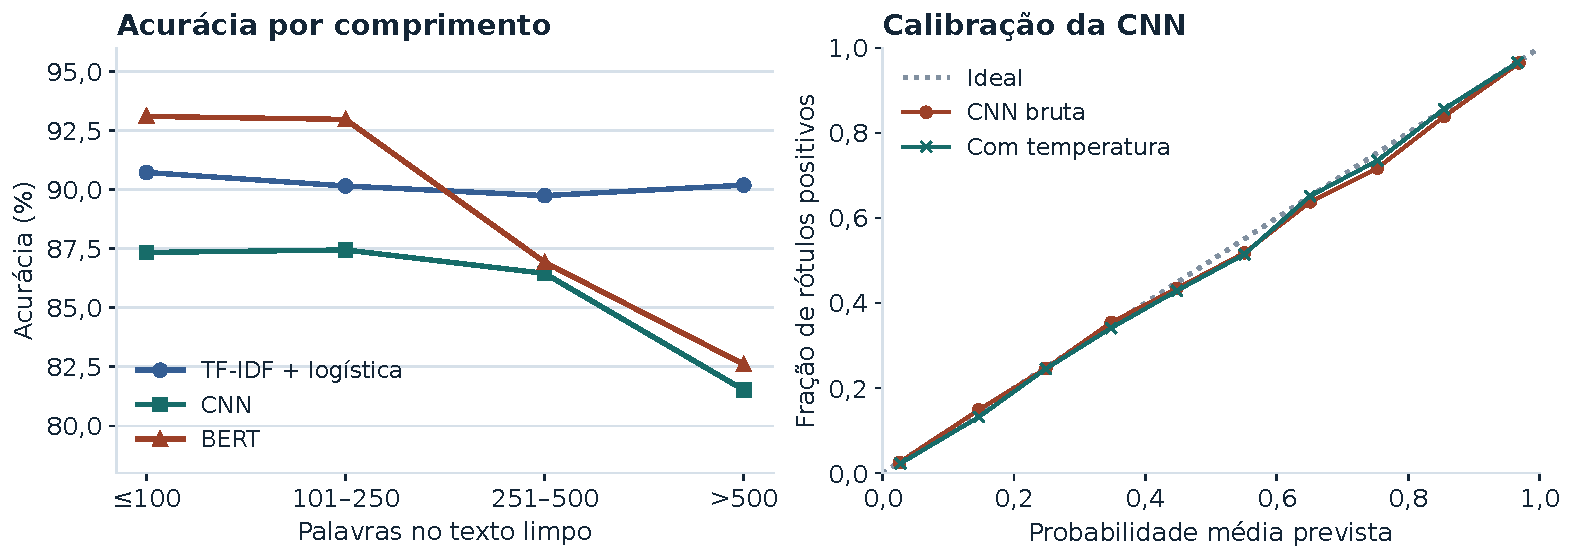
\includegraphics[width=\linewidth]{figuras/diagnostico_oficial.pdf}
\legendinha{Figura 3. À esquerda, as faixas de comprimento têm 3.246,
14.624, 5.285 e 1.845 resenhas. À direita, o eixo horizontal mostra a
probabilidade média prevista e o vertical mostra a fração de positivos
observada entre resenhas na mesma faixa de probabilidade. A diagonal
indica coincidência entre as duas medidas.}

A temperatura mudou pouco a CE da CNN, de 0,3040 para 0,3037. A acurácia
da CNN cai de 87,34\% nas resenhas de até cem palavras a 81,52\% acima
de 500. BERT também cai na faixa longa. O TF-IDF recebe o texto
completo e varia menos. Comprimento, conteúdo e recorte variam juntos.
\fonte{results/analysis/subgroup_metrics.csv}{Métricas por faixa}.

\subsection{O custo das três receitas originais}
\begin{tabularx}{\linewidth}{@{}Xlrr@{}}
\toprule
\tabelahead{Modelo} & \tabelahead{Dispositivo} & \tabelahead{Ajuste (s)} &
\tabelahead{Inferência (s)}\\
\midrule
\LinhasCusto
\bottomrule
\end{tabularx}
\legendinha{Tabela 7. A inferência soma as quatro divisões. O ajuste
do baseline inclui TF-IDF e seleção da regularização. Cada tempo vale para
o dispositivo e o orçamento da receita medida.}

\subsection{Ensaios complementares}
Em 64 enredos, o Qwen3-8B recebeu uma intervenção no bloco 28, após o
marcador de opinião. O próprio modelo reconheceu os dois tons-alvo em
55 enredos. Os resumos factuais coincidiram, mas uma opinião acrescentou
um cenário ausente da fonte \cite{qwen}.
\fonte{QWEN_EXPERIMENTO.md}{Protocolo de geração}.
O suplemento reúne 51 treinos de MLP e 880 condições sintéticas para
estudar \textit{double descent}.
\fonte{docs/CONEXOES_DISCIPLINA.md}{Guia dos mecanismos}.
